%%-----------------------------------------------------------------------
% Loading the packages and classes
%%-----------------------------------------------------------------------

\documentclass[12pt,twoside,a4paper,final]{book}%
\usepackage{a4}%                        %% Verwendet mehr Platz auf einer A4 Seite als Option a4paper in book
\usepackage[english,ngerman]{babel}%    %% Babel Sprachen
\usepackage[latin1]{inputenc}%          %% input encoder f�r umlaute usw.
\usepackage[T1]{fontenc}
\usepackage{amssymb}%                   %% AMS Symbole
\usepackage{amsmath}%                   %% AMS Math Funktionen
\usepackage{amsfonts}%
\usepackage[Sonny]{fncychap}%           %% Chapter Style
\usepackage[english,noprefix]{nomencl}%  %% Nomenclature (Symbolverzeichnis)
\usepackage{makeidx}%                   %% Index
\usepackage{graphicx}%                  %% Graphiken
\graphicspath{{img/}}
\DeclareGraphicsExtensions{.pdf,.jpeg,.png,.jpg}
\usepackage{psfrag}%                    %% Tex-Schriftarten und Formeln in EPS-Grafiken
\usepackage{color}
\usepackage{nicefrac}
\usepackage{ifthen}
\usepackage{fancyhdr}
\usepackage{subfigure}
\usepackage[xindy, acronym, toc]{glossaries}
\usepackage{cite}
\usepackage{listings}
\usepackage{color}
\usepackage[dvipsnames]{xcolor}
\usepackage{rotating}
%Define Acronyms like
% use on every place in your document \gls{mas} for TGM or - for plural - use \glspl for TGMs
% at the first usage of this, the acronym will be introduced, everywhere else it will only be the in the short form: ``Technologisches Gewerbemuseum (TGM)''
% TIPP: USE THIS FOR EVERY NAME/SOFTWARE-TOOL/MAIN PART OF YOUR WORK, like JAVA, - so that, e.g. JAVA is not written Java everywhere else in your thesis.
\newacronym{tgm}{TGM}{Technologischem Gewerbemuseum}
\newacronym{fp}{FP-Analyse}{Function-Point-Analyse}
\newacronym{afa}{AFA}{Abschreibung f�r Abnutzung}

\newacronym{ma}{MA}{Moving Average}
\newacronym{macd}{MACD}{Moving Average Convergence/Divergence}
\newacronym{cci}{CCI}{Commodity Channel Index}
\newacronym{rsi}{RSI}{Relative Strength Indicator}

\newacronym{forex}{FOREX}{Foreign Exchange Market}

\newacronym{bts}{BTS}{Backtesting-Software}
\newacronym{git}{GIT}{GIT-Server}
\newacronym{dde}{DDE}{Dynamic Data Exchange}
\newacronym{ide}{IDE}{Integrated Development Environment}
\newacronym{ib}{IB}{Interactive Brokers}

\newacronym{wcf}{WCF}{Windows Communication Foundation}
\usepackage{multirow}
\usepackage{eurosym}
%%-----------------------------------------------------------------------
% Using the Hyperref-Package for PDF-Online Version
%%-----------------------------------------------------------------------

\def\usehyperref{1}

\ifnum\usehyperref=1
\usepackage[pdftex=true,
  pdftitle={Diplomarbeit},
  pdfauthor={Gottfried Koppensteiner},
  bookmarksopen,
  colorlinks,
  citecolor=blue,
  linkcolor=blue,
  breaklinks%
]{hyperref}%
\fi



%%-----------------------------------------------------------------------
% Rearranging Nomenclature
%%-----------------------------------------------------------------------


\renewcommand{\nomname}{List of symbols}
%\renewcommand{\nompreamble}{The following list only contains symbols
%  that are used continuously throughout the text. Local symbols are
%  not listed.}
\renewcommand{\nomgroup}[1]{
 \ifthenelse{\equal{#1}{A}}{\item[\textbf{General symbols}\bigskip]}{
 \ifthenelse{\equal{#1}{B}}{\item[\bigskip\bigskip\textbf{Chapter 2}\bigskip]}{
 \ifthenelse{\equal{#1}{C}}{\item[\bigskip\bigskip\textbf{Chapter 3}\bigskip]}{
 \ifthenelse{\equal{#1}{D}}{\item[\bigskip\bigskip\textbf{Chapter 4}\bigskip]}{
 \ifthenelse{\equal{#1}{E}}{\item[\bigskip\bigskip\textbf{Chapter 5}\bigskip]}{
 \ifthenelse{\equal{#1}{F}}{\item[\bigskip\bigskip\textbf{Appendix}\bigskip]}{
 }}}}}}}
\makenomenclature



%%-----------------------------------------------------------------------
% Makes Bibliography available in Winedt
%%-----------------------------------------------------------------------

%GATHER{bib_kiefer.bib}


%%-----------------------------------------------------------------------
% Definition of possible environments
%%-----------------------------------------------------------------------

\newtheorem{theorem}{Theorem}[chapter]
\newtheorem{acknowledgement}{Acknowledgement}[chapter]
\newtheorem{algorithm}{Algorithm}[chapter]
\newtheorem{axiom}{Axiom}[chapter]
\newtheorem{case}{Case}[chapter]
\newtheorem{claim}{Claim}[chapter]
\newtheorem{conclusion}{Conclusion}[chapter]
\newtheorem{condition}{Condition}[chapter]
\newtheorem{conjecture}{Conjecture}[chapter]
\newtheorem{corollary}{Corollary}[chapter]
\newtheorem{criterion}{Criterion}[chapter]
\newtheorem{definition}{Definition}[chapter]
\newtheorem{example}{Example}[chapter]
\newtheorem{exercise}{Exercise}[chapter]
\newtheorem{lemma}{Lemma}[chapter]
\newtheorem{notation}{Notation}[chapter]
\newtheorem{problem}{Problem}[chapter]
\newtheorem{proposition}{Proposition}[chapter]
\newtheorem{remark}{Remark}[chapter]
\newtheorem{solution}{Solution}[chapter]
\newtheorem{summary}{Summary}[chapter]
\newenvironment{proof}[1][Proof]{\noindent\textbf{#1.} }{\ \rule{0.5em}{0.5em}}

\renewcommand{\chaptermark}[1]{\markboth{\thechapter.\ #1}{}}
\renewcommand{\sectionmark}[1]{\markright{\thesection.\ #1}}




%%-----------------------------------------------------------------------
% Marking of overfull boxes and increasing of tolerances
%%-----------------------------------------------------------------------

% F�r die Final-Version die n�chste Zeile auskommentieren um schawarze Balken (TU-Logo im Titelblatt) zu ignorieren!
\overfullrule=10pt%                     %% Markiert �berf�llte Boxen. z.b. hbox overfull (Evtl. nicht im pdf sichtbar!!!!)
\hfuzz=1pt%                             %% Toleranz bei hbox overfull erh�ht 1pt entspr. ca. 1/3 mm


%%-----------------------------------------------------------------------
% Counter
%%-----------------------------------------------------------------------


\setcounter{secnumdepth}{3}%
\setcounter{tocdepth}{3}%



% Clear Header Style on the Last Empty Odd pages
\makeatletter
\def\cleardoublepage{\clearpage\if@twoside \ifodd\c@page\else%
    \hbox{}%
    \thispagestyle{empty}%              % Empty header styles
    \newpage%
    \if@twocolumn\hbox{}\newpage\fi\fi\fi}
\makeatother

%%-----------------------------------------------------------------------
% Avoid indents
%%-----------------------------------------------------------------------

\setlength{\parindent}{0pt}

%%-----------------------------------------------------------------------
%% Hyphenation for german abstract
%%-----------------------------------------------------------------------

\hyphenation{Fa-mi-lie
             Ski-bil-dung
             Ar-beits-wal-ze
             neg-lec-ted
             se-par-ate
             di-men-sio-nal
             her-r\"uhren
             N\"a-herungs-l\"os-ungen
             wissen-schaft-licher
             Regelungs-technik
             re-con-fi-gur-abili-ty
             manage-ment
             manu-facturing
             not-wendigen
             }


%%-----------------------------------------------------------------------
% Colored grafix
% 1 = color
% 0 = grey
%%-----------------------------------------------------------------------


\def\colorsw{1}

%%-----------------------------------------------------------------------
% Additional remarks
% 1 = with remarks
% 0 = without remarks
%%-----------------------------------------------------------------------


\def\addnotes{0}


%%-----------------------------------------------------------------------
% Define month
%%-----------------------------------------------------------------------

\def\monthdis{Oktober 2012}

\makeglossaries
%%-----------------------------------------------------------------------
% Document
%%-----------------------------------------------------------------------


\begin{document}%
\selectlanguage{ngerman}%
\renewcommand{\indexname}{Index}%
\topmargin15.0mm


\def\tpdefault{{\sf \center \vspace*{-4cm}
%\begin{center}
%\hspace*{-1.3cm}
%\rule{17cm}{0.02cm}
%\end{center}


\begin{figure}[h]
\begin{flushright}	
		
\includegraphics[width=0.3\textwidth]{graphics/title/tgmlogo2.png}
	\label{fig:tgmlogo}
\end{flushright}
\end{figure}


\vspace{2cm}


{\Large %\bf 
Machbarkeitsstudie\\ \vspace{0.7cm}}
 {\LARGE \sloppy
{\bf \sf  \textbf{AQUILA \\}
Tradingsoftware mit Webschnittstelle
\\}}
%
%
\vspace*{2cm}
{\normalsize Ausgef\"uhrt in Zuge des Projektmanagement-Unterrichts im 5. Jahrgang\\
Ausbildungszweig Systemtechnik/Medientechnik\\ %unzutreffendes streichen
  \vspace{1.5cm}
  \normalsize unter der Leitung von\\
  \large Prof.\ Mag.\ Hans Brabenetz\\
  \normalsize Abteilung f�r
  Informationstechnologie\\
  \vspace{1.5cm}
  eingereicht am  Technologischen Gewerbemuseum Wien\\
  H\"ohere Technische Lehr- und Versuchsanstalt\\
  Wexstrasse 19-23, A-1200 Wien\\
  }}}


\begin{titlepage}
	\tpdefault
	{\sf \center \vspace{1.0cm}
	\normalsize von\\
	\large 
	Peer Nagy 5CHITI\\
	Gabriel Pawlowsky, 5BHITS\\
	Josef Sochovsky, 5BHITS\\
	\vspace {2 cm}
	\bf \sf {Wien, im \monthdis} \\
		%	\vspace{2cm}
	%	\rule{\textwidth}{0.01cm}
	
	}



	\end{titlepage}
\frontmatter%   %% front matter will be numbered in small Roman letters

%%-----------------------------------------------------------------------


%TCIDATA{OutputFilter=latex2.dll}
%TCIDATA{Version=5.00.0.2552}
%TCIDATA{LaTeXparent=0,0,Dissertation_SW.tex}


\chapter*{Vorwort}

Diese Arbeit wurde im Jahr 2012 im Zuge unserer Ausbildung in der Abteilung f�r Informationstechnologie am \gls{tgm}, HTBLVA Wien 20, durchgef�hrt. 


\bigskip

Dankesworte

\bigskip
\bigskip
\bigskip
\bigskip



Wien, im \monthdis \hfill Name, Name, Name, Name \vfill
%
\selectlanguage{english}%
\chapter*{Abstract}

This is the english abstract.%
\selectlanguage{ngerman}%
\chapter*{Kurzfassung}

Deutsche Kurzfassung kommt hierher%


%%-----------------------------------------------------------------------
% Define Header for Content chapter
%%-----------------------------------------------------------------------


\makeatletter
\def\tableofcontents{\chapter*{\contentsname\@mkboth{\contentsname}{\contentsname}}
  \@starttoc{toc}}
\makeatother

\clearpage%
\tableofcontents
\clearpage
\listoffigures
\clearpage
\lstlistoflistings %\listoftables
\clearpage 
\markboth{Contents}{Contents}


%\addcontentsline{toc}{chapter}{\numberline{}\listfigurename}%
%\listoffigures
%\listoftables%
%\addcontentsline{toc}{chapter}{\numberline{}\listtablename}%
\clearpage%



\nomenclature[aa]{$t$}{time}
\nomenclature[bb]{$t_0$}{reference time}
\nomenclature[aa]{$m$}{mass}
\nomenclature[aa]{$\rho$}{mass density}

\markboth{\nomname}{\nomname}%
\addcontentsline{toc}{chapter}{\numberline{}\nomname}%
\printnomenclature


\mainmatter%   %% main part will be numbered in Arabic letter


% include chapters
% !TeX root = ../Aquila_Machbarkeitsstudie.tex
% Chapter1

\chapter{Einleitung} \label{chapter:einleitung}

Aktienhandel ist meist mit viel Erfahrung verbunden. Umso kurzfristiger gehandelt wird, desto mehr Konzentration und Aufmerksamkeit muss den Vorg�ngen gewidmet werden, damit auch bei mehreren Trades am Tag summa summarum eine positive Bilanz entsteht. Dies macht es f�r kleine Firmen schwierig und f�r handelnde Privatpersonen nahezu unm�glich in diesem Zeitraum zu operieren. Das Ziel dieses Projektes ist es, genau bei dieser Zielgruppe zu punkten, indem eine Software zur algorithmischen Abbildung eines Handelssystems geschaffen wird, die automatisch Kauf- und Verkaufentscheidungen trifft. Eine Website als Schnittstelle zum Benutzer gew�hrleistet Plattformunabh�ngigkeit, gibt Informationen �ber Performance und Preisentwicklungen und erm�glicht das �ndern von Parametern von �berall. Zus�tzlich k�nnen mehrere Benutzer von unterschiedlichen Standorten mit einem gemeinsamen Portfolio operieren.\\
	Charts auf der Website bieten live einen �berblick �ber die aktuelle Situation und dadurch eine erh�hte Transparenz der Arbeitsweise und Entscheidungsgenerierung des Algorithmus. Relevante Parameter, wie die zu handelnden Aktien oder die H�he der Investition k�nnen ebenfalls einfach �ber die Webschnittstelle ver�ndert werden.%
% !TeX root = ../Aquila_Pflichtenheft.tex

% Chapter2: Produkteinsatz

\chapter{Produkteinsatz} \label{chapter:produkteinsatz}
\section{Anwendungsbereiche und Zielgruppen}

Das Produkt implementiert ein Handelssystem f�r Aktien. Daher ist f�r einen vern�nftigen Umgang mit der Software ein Mindestwissen �ber Aktienhandel und B�rsengesch�fte vorauszusetzen. Vorteilhaft w�re ebenso ein Verst�ndnis von technischer Analyse und h�ufig genutzten Indikatoren, um darauf basierende Handelssysteme zu durchschauen. Programmier- b.z.w. vertiefende Computerkenntnisse m�ssen hingegen nicht vorhanden sein.\\
	Als Zielgruppe sind insbesondere kleine und mittlere Unternehmen (KMU) anvisiert, in denen sich bereits Personen mit finanzwirtschaftlichen Angelegenheiten befassen. Hinzu kommen private Einzelpersonen, die �ber das n�tige Kapital f�r kurzfristigen Aktienhandel verf�gen und mit wenig Aufwand ein Komplettsystem dazu anwenden m�chten.

\section{Betriebsbedingungen}

Die Software soll es prinzipiell erm�glichen unbeaufsichtigt und selbstst�ndig zu arbeiten, wobei, da es sich um einen substanziellen Kapitalaufwand handeln kann, es insbesondere in der Anfangszeit ratsam ist, die Abl�ufe der Software zu �berwachen.\\
	Sowohl die Handelssoftware selbst als auch die Webseite laufen auf einem Server. Beide Komponenten m�ssen die Aufteilung auf und somit die Kommunikation zwischen mehreren Servern nicht unbedingt unterst�tzen, jedoch w�re dies vorteilhaft, da sowohl Zugriffsrechte separat geregelt werden k�nnten, als auch die Handelssoftware die vollen Kapazit�ten des Servers nutzen kann.\\
	Software und Website sollen einen Betrieb rund um die Uhr erm�glichen, ob ein solcher im Einsatz tats�chlich realisiert wird, liegt am Kunden.%
% Chapter3

\chapter{Produktumgebung} \label{chapter:Produktumgebung}

\section{Software}
\label{software}

Um das Ausf�hren der Software zu gew�hrleisten, ist es n�tig einen Webservice anbieten zu k�nnen. Weil das Teilprodukt, die Website, haupts�chlich mit ASP.NET geschrieben ist, muss einer der folgenden Webservern lauff�hig installiert sein:
\begin{itemize}
	\item Internet Information Services (\textbf{IIS})
	\item \textbf{Apache-Webserver} (mit \"mod\_apsdotnet\" und \"mod\_mono\")
	\item \textbf{XSP-Webserver}
	\item \textbf{Cassini-Webserver}
\end{itemize}
Im Falle, dass ein Linuxserver f�r die Website benutzt werden soll wird ein Apache oder der XSP-Webserver empfohlen, damit es zu keinen schwerwiegenden Problemen f�hren kann.
\\
Es wird angeboten die Website und die Software auf unterschiedlichen Computern zu installieren und dort zu benutzen.
F�r das reibungslose Integrieren der Software wird ben�tigt:
\begin{itemize}
	\item Datenbankserver	zum Interagieren mit der Website (Postgresql)
	\item ein installierter und funktionierender \textbf{\gls{ib}-Client}
	\item ein Client von e-Signal
	\item die aktuellste Version des \textbf{.NET-Frameworks}
\end{itemize}

\section{Hardware}
\label{hardware}

Im Falle \textbf{eines} Servers wird ben�tigt der Rechner auf jeden Fall 4 GB Arbeitsspeicher, zirka 100GB freier Speicher und zumindest einen Dual-Core Prozessor.\\
Allerdings liegen diese Werte bereits unter dem heutigen Standard f�r die normalen Server. Wenn man die mindeste Konfiguration w�hlt wird empfohlen keine weiteren Servert�tigkeiten �ber dieses Ger�t zu vollziehen. Es ist au�erdem eine Internetanbindung erforderlich, sowie ausreichend viel Speicherplatz auf der/den Festplatte/n.

\section{Orgware}
\label{orgware}
Der Server, auf dem die Software und die Website verwenden wird, muss mit dem Internet verbunden sein, damit er sich mit \gls{ib}und e-Signal verbinden kann. Dazu wird zuz�glich ein Account dieser beiden Anbieter ben�tigt.%
% Chapter4
\chapter{Produktfunktionen} \label{chapter:thevetestcase}

\begin{quotation}
``The market is not an invention of capitalism. It has existed for centuries. It is an invention of civilization.``
\begin{flushright}
(Mikhail Gorbachev)
\end{flushright}
\end{quotation}%
% Chapter5

\chapter{Wirtschaftliche Machbarkeit} \label{chapter:Wirtschaftliche Machbarkeit}

\section{Aufwandsabsch�tzung}

\begin{figure}[h]
	\centering
		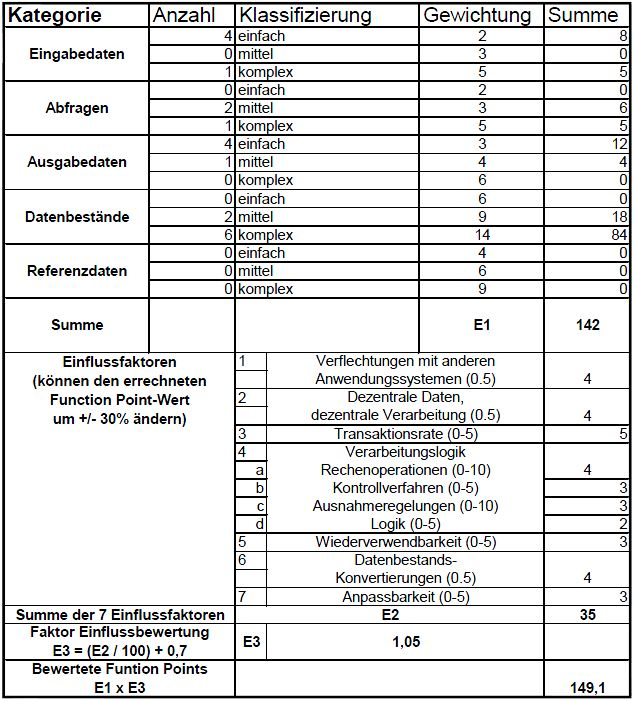
\includegraphics{graphics/chapter5/FunctionPointsAnalysis.JPG}
	\label{fig:FunctionPointsAnalysis}
\end{figure}


\section{Risikoanalyse}
\label{section:Risikoanalyse}

\subsection{Personenausfall}
\label{subsection:Personenausfall}

Eintrittswahrscheinlichkeit:  gering \\
Auswirkungen:  								gering \\

In dem unerwarteten Fall, dass ein Teammitglied l�ngerfristig ausf�llt, muss es m�glich sein die Arbeitsaufgaben dementsprechend neu aufteilen zu k�nnen.
Folgende F�lle k�nnten auftreten:
\begin{itemize}
	\item Streit im Team
	\item Ausfall durch Krankheit oder Tod eines Teammitglieds
	\item Austritt eines Teammitglieds aus dem Projekt
	\item Der Auftraggeber k�nnte aufgrud von Unklarheiten den Projektabbruch initiieren 
	\item Es kann passieren, dass von Seite des Auftragsgebers pl�tzlich kein Interesse an der Umsetzung des Produktes mehr gegeben ist, und es dadurch zu extremem Zeitverzug kommt, was bis zum Abbruch f�hren kann
\end{itemize}

Folgende pr�ventive Ma�nahmen werden eingef�hrt:
\begin{itemize}
	\item Regeln f�r den Umgang innerhalb des Projekts
	\item Ausreichendes Interesse jedes Mitglieds und keine leistungstechnische Probleme 
	\item Gutes Verh�ltnis mit den Auftraggebern
\end{itemize}

\subsection{Zetiliche Risiken}
\label{subsection:Zeitliche Risiken}

Eintrittswahrscheinlichkeit:  gering \\
Auswirkungen:  								mittel \\

Die Aufwands- und Zeitsch�tzung basiert auf dem derzeitigen Lastenheft des Auftraggebers und stellt eine zeitgerechte Fertigstellung sicher. Sollten sich jedoch die Anforderungen des Kunden w�hrend des Projekts �ndern, so wird sich das mit gro�er Wahrscheinlichkeit verz�gernd auf den Fertigstellungstermin auswirken. Die mit dem Kunden vereinbarte Funktionsanalyse und die Meilensteine mit gemeinsam festgelegten Qualit�tskriterien sollten jedoch diesem Risiko entgegenwirken.

\subsection{Technische Risiken}
\label{subsection:Technische Risiken}
\textbf{Datenverlust}\\
Eintrittswahrscheinlichkeit:  gering \\
Auswirkungen:  								mittel \\

Aufgrund der nicht auszuschlie�enden Gefahr des Datenverlusts, muss daf�r gesorgt werden die Sicherheit der Daten, sowie auch die Verf�gbarkeit dieser zu garantieren. Dieses Problem wird mithilfe eines \gls{git} gel��t, durch diesen Server ist es m�glich die Versionen der Software immer zug�nglich zu machen und zus�tzlich die Daten auf den Computern der Projektmitgliedern zu speichern.


\section{Kosten / Nutzenpotential}

* Was k�nnte an Umsatz entstehen?
* Lizensierung des Gesamtpaketes	->	Softwareverkauf + Installation der Webseite
* Kosten aus FP-Analyse gegenrechnen

Das Ziel des Projektes Aquila ist es einerseits eine Variante zur Automatisierung des Aktienhandels zu schaffen und dabei die volle Kontrolle und �bersicht zu behalten. Andererseits liegt ein langfristiger Nutzen in der Entstehung von Knows-How und der technischen Fortbildung des Projektteams; schlie�lich ist das Kapital Bildung bei der Abw�gung des Nutzens nicht au�er Acht zu lassen.\\
Die Tradingsoftware samt Website zur Steuerung dieser soll als einfach zu bediendes Komplettpaket angeboten werden. Die Nutzungs- und Vertriebsrechte bleiben bei den Entwicklern, verkauft werden k�nnen Lizenzen mit beliebig beschr�nkter Nutzerzahl zu unterschiedlichen Preisen.\\
*zB: Einzellizenz, 5-Benutzer, Unlimited
Ebenfalls in Rechnung gestellt wird die Installation der Software auf einem entweder bereits verf�gbaren System oder es wird die ben�tigte Serverarchitektur gemietet. Das Service der Serverbereitstellung ist von Auftragnehmerseite nicht vorgesehen. Sollte dies allenfalls gew�nscht werden, wird das Hosting vermutlich outsourced gemanaged.\\
Die Trading-Software trifft vollst�ndig automatisiert Entscheidungen zum Kauf und Verkauf von Wertpapieren und erm�glicht es somit auch potentiellen Marktteilnehmern mit wenig Zeit systemisch zu handeln, was ohne Software mit erheblichem Zeitaufwand einhergeht. Die Software bleibt dabei ebenfalls stets ver�nder- und erweiterbar; Kunden k�nnten zuk�nftige, neue Softwareversionen gegen Abopreis verrechnet, beim Initialkaufpreis einberechnet oder einzeln verkauft werden. Die Website erm�glicht das gesamte Controlling der Software und bietet neben Konfiguration der Handelseigenschaften �berblick �ber aktuelle Vorg�nge. \\
Die Software ist auf das Handeln �ber einen Broker-Account ausgelegt, wodurch eine Zielgruppe von privaten oder institutionellen Einzeltradern oder kleinen Tradinggruppen angesprochen werdeb. Ebendiese Zielgruppe profitiert besonder von der Simplizit�t der Verwaltung, der �bersicht und des Erweiterungs- und Verbesserungspotentials.%
\chapter{Produktleistungen} \label{chapter:Produktleistungen}

%


\addcontentsline{toc}{chapter}{Glossary} 
\printglossary[type=\acronymtype]
\glsaddall

\printglossary[type=\acronymtype]
%\printglossary[type=\acronymtype,style=listwithwidth]

%% include appendix
\begin{appendix}
\chapter{Appendix\label{appendix_A}}
%
\end{appendix}

% Use of the sorted IEEE style, with changes:
% "dashification" was disabled


\cleardoublepage

% IEEE Style
\bibliographystyle{sty/IEEEtranS}

% GATHER
%\input "bib_file.bib"
\phantomsection{}
\addcontentsline{toc}{chapter}{\bibname}
\pagestyle{myheadings}\markboth{\bibname}{\bibname}
\bibliography{tex/bib_file}

%%% generate index
%\clearpage%
%\markboth{\indexname}{\indexname}%
%\printindex%
%\addcontentsline{toc}{chapter}{\numberline{}\indexname}%

%% include affidavit
\thispagestyle{empty}
\vspace*{2cm}
\begin{center}
{\bf \sf \huge Erkl{\"a}rung}
\end{center}
{\sf \vspace{1cm} Hiermit erkl{\"a}ren wir, dass die vorliegende
Arbeit ohne unzul{\"a}ssige Hilfe Dritter und ohne Benutzung
anderer als der angegebenen Hilfsmittel angefertigt wurde. Die aus
anderen Quellen oder indirekt �bernommenen Daten und Konzepte sind
unter Angabe der Quelle gekennzeichnet.

Die Arbeit wurde bisher weder im In- noch im Ausland in gleicher
oder in {\"a}hnlicher Form in anderen Pr{\"u}fungsverfahren
vorgelegt.
\\[1.5cm]
Wien, im \monthdis
\\[2cm]
Name1
\\[2cm]
Name2
\\[2cm]
Name3
\\[2cm]
Name4
\\[2cm]
}%end sf
%



\end{document}
%%%%%%%%%%%%%%%%%%%%%%%%%%%%%%%%%%%%%%%%%%%%%%%%%%%%%%%%%%%%%%%%%%%%%%%%%%%%%%%%%%%%%%%%%%%%%%%%%%%
%%%%%%%%%%%%%%%%%%%%%%%%%%%%%%%%%%%%%%%%%% End Dokument %%%%%%%%%%%%%%%%%%%%%%%%%%%%%%%%%%%%%%%%%%%
%%%%%%%%%%%%%%%%%%%%%%%%%%%%%%%%%%%%%%%%%%%%%%%%%%%%%%%%%%%%%%%%%%%%%%%%%%%%%%%%%%%%%%%%%%%%%%%%%%%
